\section{The Stokes Equations in NGSolve}

The Stokes Equations are linear partial differential equations, which describe a stationary incompressible Newtonian fluid flow
with high viscosities and low Reynolds numbers. For the implementation in NGSolve, a suitable geometry and boundary conditions are 
the ones proposed by Sturm et. al. \cite{nearly_conformal_paper}, where the fluid flow around a cylinder is investigated while the
outer boundary of $\Omega$ is prescriped a velocity striclty in $x$ direction, the so called far field velocity:

\null

\begin{figure}[!htbp]
\begin{minipage}{.5\textwidth}
    \centering
    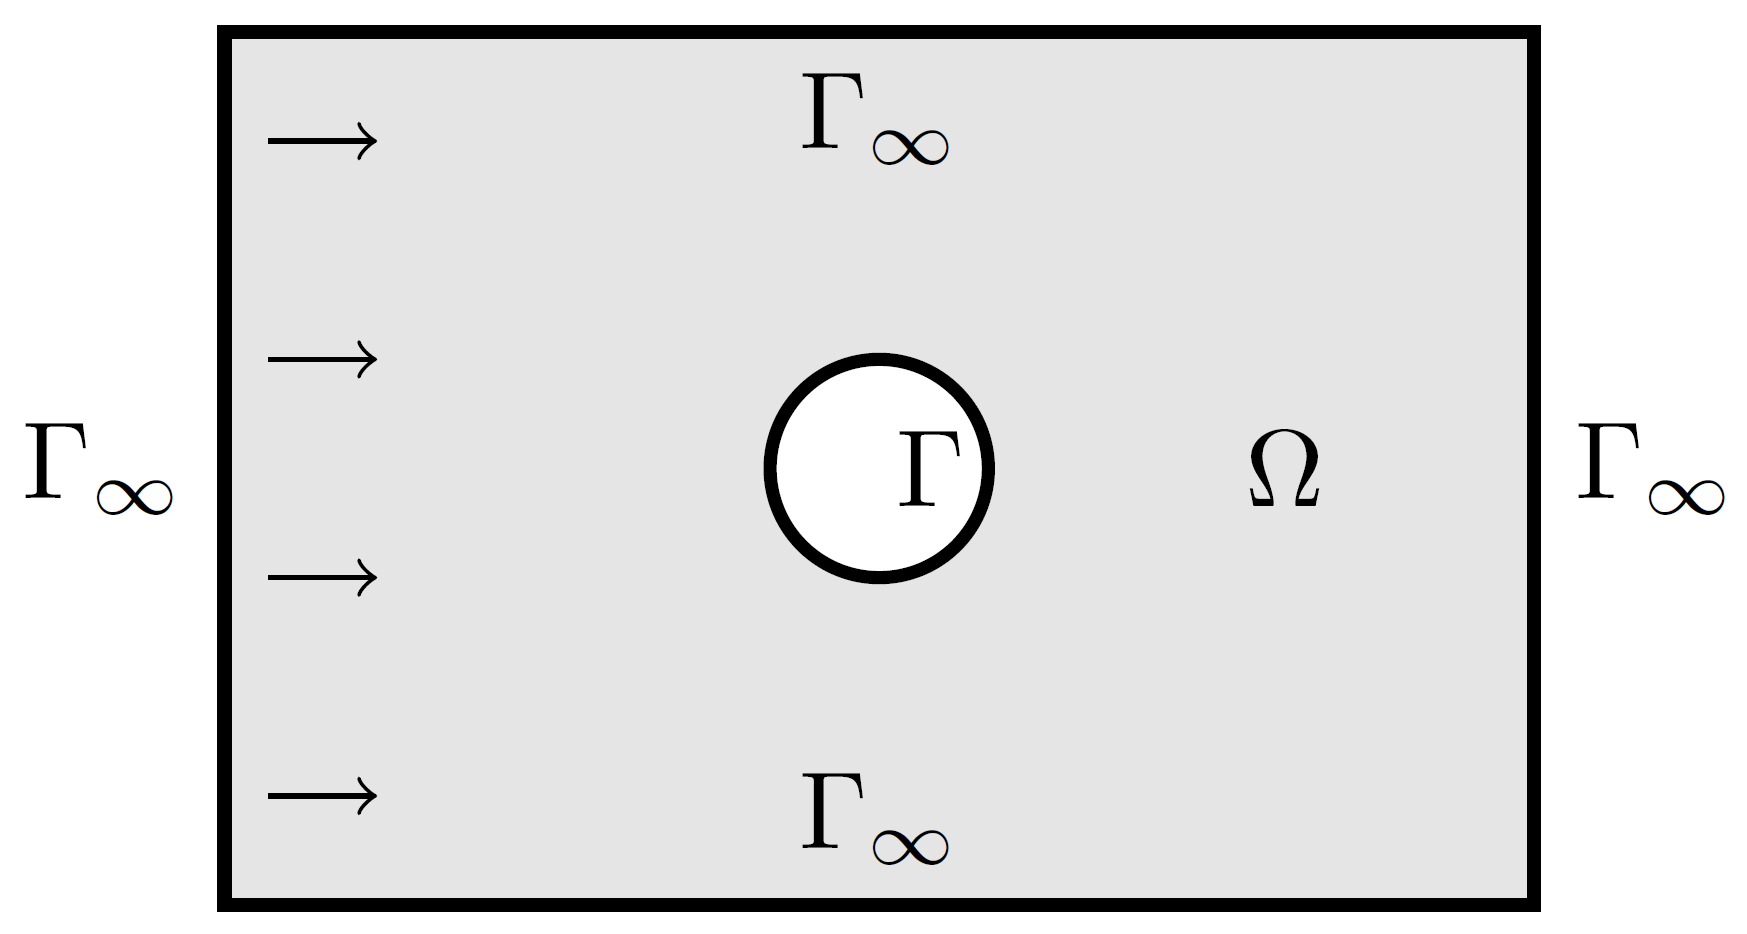
\includegraphics[width=0.8\textwidth]{figures/domain_graphic_sturm.PNG}
    \caption{Domain $\Omega$ for Stokes PDE's (\ref{stokes_PDE}) \cite{nearly_conformal_paper}}
    \label{domain_graphics}
\end{minipage}
\begin{minipage}{.5\textwidth}
    \begin{equation}\label{stokes_PDE}
        \begin{aligned}
            -\mu \Delta u + \nabla p &=0& \, &\text{in } \Omega,& \\
            \mathrm{div} \, u &=0& \, &\text{in } \Omega,& \\
            \mathbf{u} &=0& \, &\text{on } \Gamma,& \\
            \mathbf{u} &=\mathbf{u}_{\infty}& \, &\text{on } \Gamma_{\infty},& \\
        \end{aligned}
    \end{equation}
\end{minipage}
\end{figure}

\null

Where $\mu \in \mathbb{R}$ is the viscosity constant and is set to 1 for simplicity. 
The problem yields the vectorial velocity field $u:\Omega \rightarrow \mathbb{R}^d$ and 
the scalar pressure field $p:\Omega \rightarrow \mathbb{R}$. In order to solve the Stokes equation with the Finite Element Method in NGSolve,
it needs to be transformed to the weak formulation, where the solutions $u$ and $p$ are linear combinations of basis functions in a Sobolev space.
See Faustmann\cite{lecture_notes_faustmann_numPDE} Chapter 3 for further elaborations on Sobolev spaces. The weak formulation can be derrived by
multipling the now called trial-functions $u$ and $p$ with test-functions $v$ and $q$, perform transformations and integrate them. The test-functions have to fulfil certain
conditions to permit the transformations in order to arrive at a weak problem with 
linear convergence rates, see Faustmann\cite{lecture_notes_faustmann_numPDE}: \\

Find $u \in [H^1_0(\Omega)]^d$ and $p \in L^2(\Omega)$ such that
\begin{equation}\label{weak_stokes_PDE}
    \begin{aligned}
    &\int_{\Omega} \nabla u : \nabla v \, dx + \int_{\Omega} \mathrm{div}(v)p \, dx &=& \, 0 &\forall& v \in [H^1_0(\Omega)]^d \\
    &\int_{\Omega} \mathrm{div}(u)q \, dx &=& \, 0   &\forall& q \in L^2(\Omega)
    \end{aligned}
\end{equation}

\null

Instead of considering this as a system of equations, one can look at the mixed method as one variational problem on
the product spaces $[H^1_0(\Omega)]^d \times L^2(\Omega)$, this is done by just adding both problems \cite{lecture_notes_faustmann_numPDE}:

\null

\begin{equation}\label{weak_stokes_PDE_product}
    \int_{\Omega} \nabla u : \nabla v \, dx + \int_{\Omega} \mathrm{div}(v)p \, dx + \int_{\Omega} \mathrm{div}(u)q \, dx = \, 0 \quad \forall (v,q)
    \in  [H^1_0(\Omega)]^d \times L^2(\Omega)
\end{equation}

\null

In lines 19-26 of listing \ref{basic_stokes}, the variational problem \ref{weak_stokes_PDE_product} is added to
a \texttt{BilinearForm()}. After assembling of the system, in line 27-31 the non-zero Dirichlet conditions are assigned. 
When setting up the geometry, the boundaries already have to be named to do the boundary conditions assignment. The geometry
shown in figure \ref{domain_graphics}, is defined in the beginning in lines 5-11.


\pagebreak

\begin{lstlisting}[language=Python, title=Basic Stokes PDE's with Python3 and NGSolve, label=basic_stokes]
    k = 2
    V = H1(mesh,order=k, dirichlet="top|bot|cyl|in|out")
    Q = H1(mesh,order=k-1)
    FES = FESpace([V,V,Q])
    ux,uy,p = FES.TrialFunction()
    vx,vy,q = FES.TestFunction()
    def Equation(ux,uy,p,vx,vy,q):
        div_u = grad(ux)[0]+grad(uy)[1] # custom divergence u
        div_v = grad(vx)[0]+grad(vy)[1] # custom divergence v
        return (grad(ux)*grad(vx)+grad(uy)*grad(vy) + div_u*q + div_v*p)* dx
    a = BilinearForm(FES)
    a += Equation(ux,uy,p,vx,vy,q)
    a.Assemble()
    gfu = GridFunction(FES)
    uinf = 0.001
    uinf_c = CoefficientFunction((uinf))
    gfu.components[0].Set(uinf_c, definedon=mesh.Boundaries("in|top|bot|out"))
    def solveStokes():
    res = gfu.vec.CreateVector()
    res.data = -a.mat * gfu.vec
    inv = a.mat.Inverse(FES.FreeDofs())
    gfu.vec.data += inv * res
    scene_state.Redraw()
\end{lstlisting}

Below the solution obtained with NGSolve (see listing \ref{basic_stokes}). On the surface of the cylinder, 
the no-slip condition (standard Dirichlet = 0) can be observed. Also an intuitive observation of the fulfilled continuity can be made:
where the cross section is smaller, e.g. in $x$ vicinity of the cylinder, the velocity is increased:

\begin{figure}[ht]
    \centering
    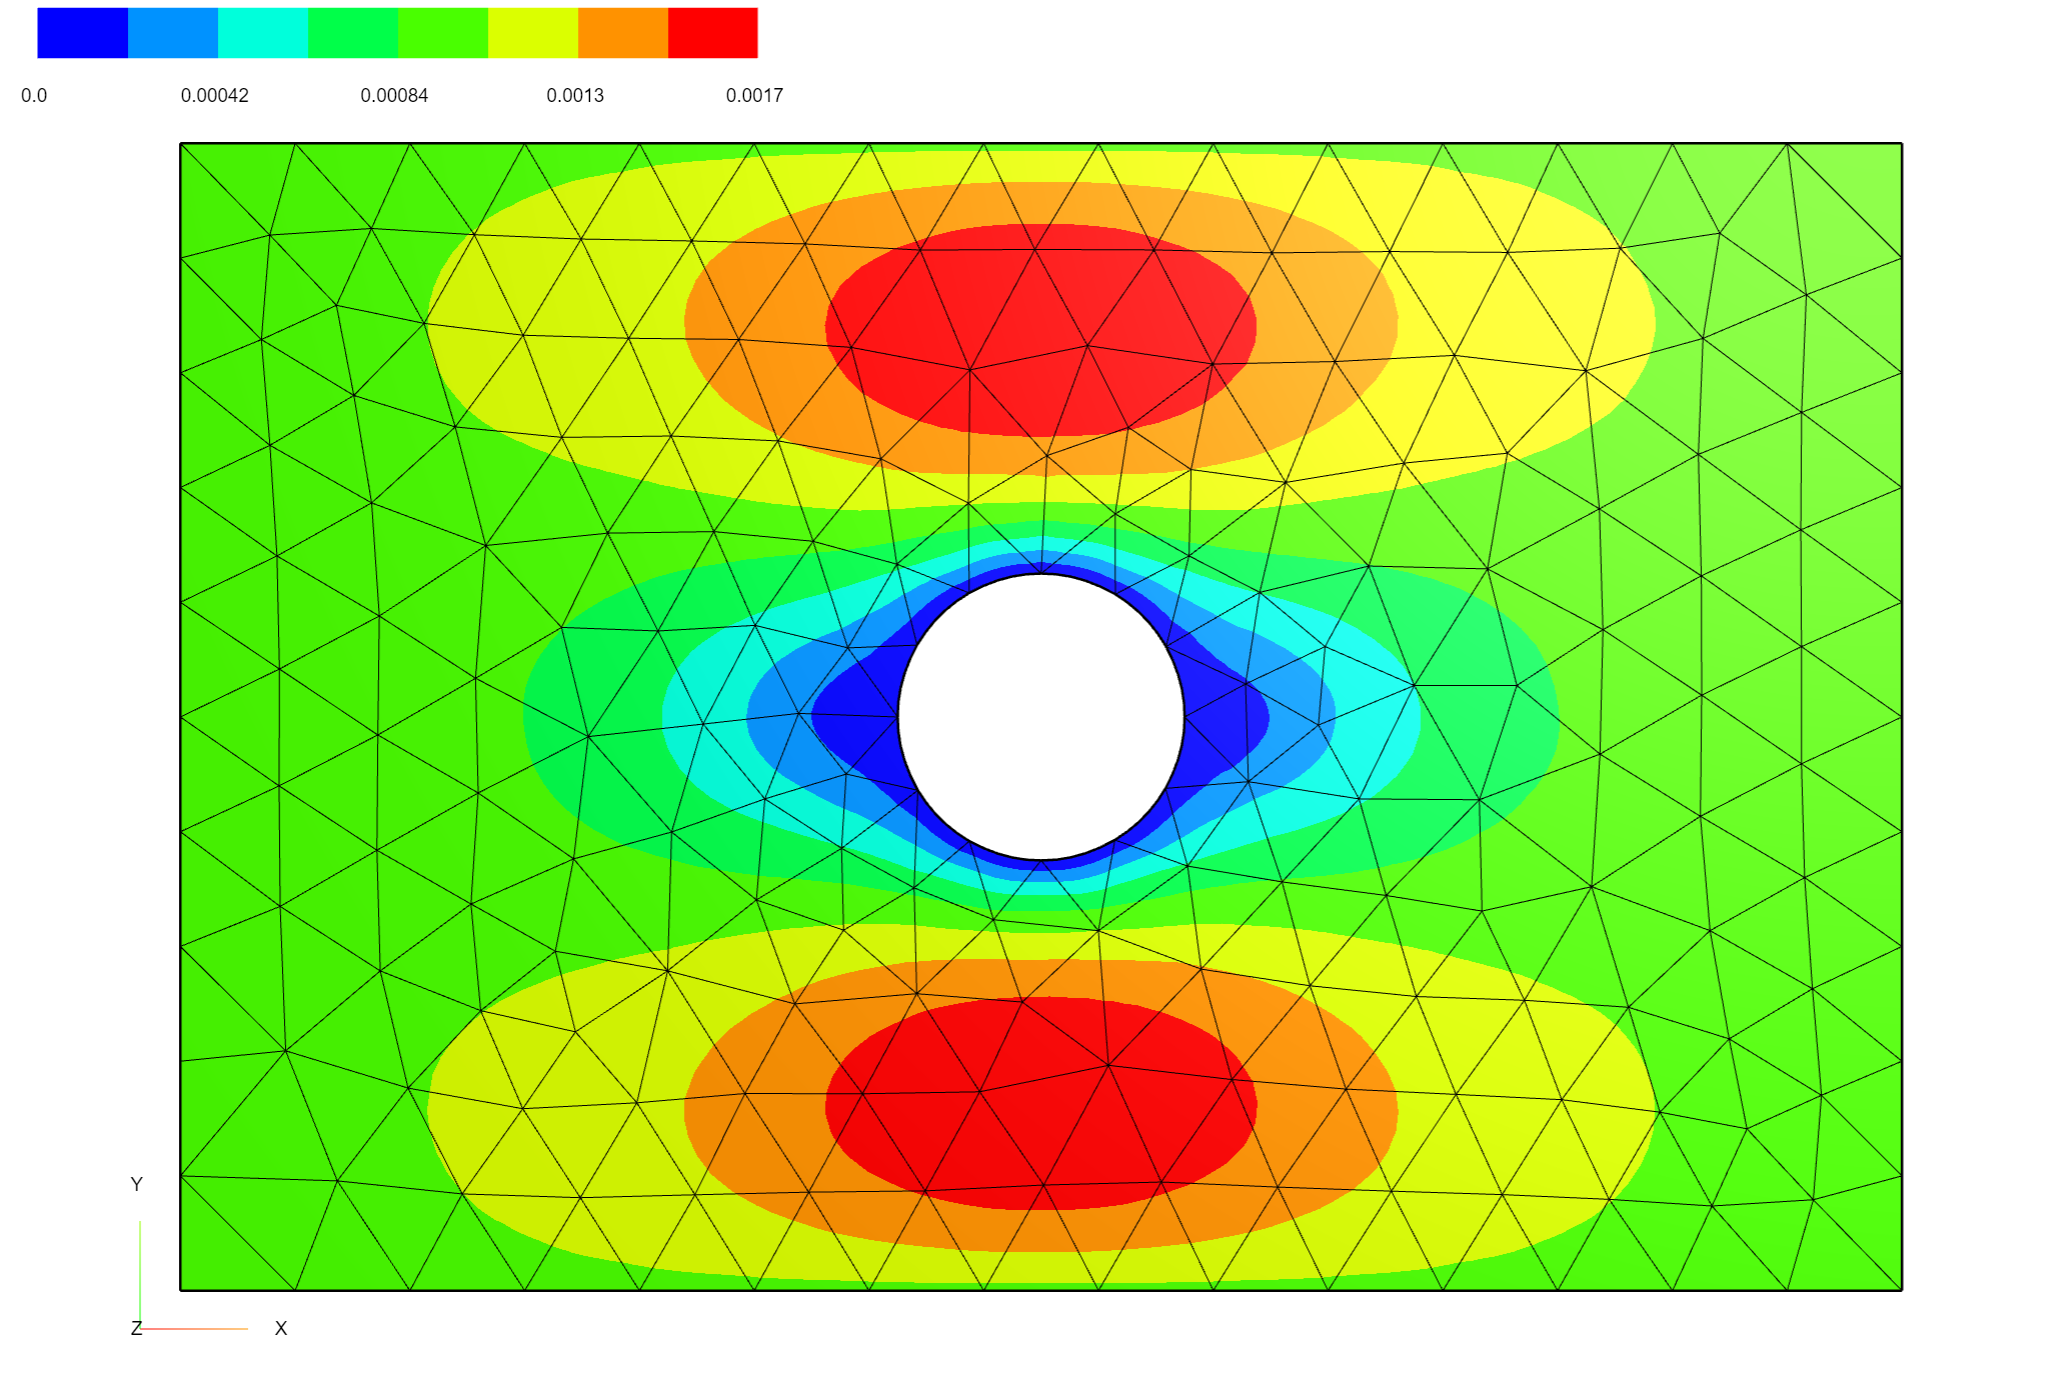
\includegraphics[width=0.92\textwidth]{figures/solution_stokes_basic.PNG}
	\caption{Surface Plot - Velocity $||\mathbf{u}||_2$ of Stokes Flow - FEM solution to problem (\ref{stokes_PDE})}
	\label{basic_stokes_flow_plot}
\end{figure}